\chapter{RandomX: a máquina que muda de ideias}
\label{chapter:randomx}
\label{page:randomx-start}

\begin{quote}
Um ASIC nasce sabendo uma profissão e, como certos cavalheiros de fortuna,
dedica o resto da vida a impedir que se note quão poucas coisas sabe fazer.
RandomX oferece-lhe uma profissão nova a cada tentativa.
\end{quote}

No capítulo anterior deixámos o mineiro diante de uma condição curta. Dado o
objecto de hash de um bloco, uma dificuldade \(d\) e um resultado de prova de
trabalho \(h_{\rm PoW}\), o bloco passa quando
\begin{align}
 h_{\rm PoW}\,d\leq 2^{256}-1.
 \label{eq:randomx-difficulty-check}
\end{align}
Nada nessa desigualdade diz quanto custa produzir \(h_{\rm PoW}\). Uma função
hash vulgar faz sempre a mesma sequência de operações. Um circuito construído
para essa sequência pode deitar fora tudo o que não usa e repetir o resto com
uma eficiência que um processador geral dificilmente alcança. A matemática do
alvo continua impecável; a economia de quem o procura mudou de dono.

RandomX é a função de prova de trabalho activa em Monero desde a versão 12.
Foi desenhada para estreitar a vantagem entre processadores de uso geral e
máquinas especializadas. Em vez de pedir a cada tentativa a mesma receita,
gera programas imprevisíveis, executa-os numa máquina virtual, movimenta um
conjunto grande de memória e condensa o estado final num hash de 256 bits
\cite{randomx-spec-v1,randomx-design-v1}. O nome vem daí: execução aleatória.

Convém declarar já a modéstia da promessa. RandomX não demonstra que um ASIC é
impossível, nem identifica uma essência metafísica chamada «CPU». Prende o
trabalho a uma colecção ampla de recursos que os processadores correntes já
possuem: aritmética inteira, vírgula flutuante, registos, vários níveis de
memória, saltos, execução especulativa e largura para instruções independentes.
Uma máquina especializada pode reproduzi-los; a esperança é que, ao terminar,
tenha pago por grande parte de um processador.

Este capítulo não reproduz programas, instruções de montagem ou funções do
código. Trataremos RandomX como tratámos uma assinatura: entradas, estado,
transformações e condições de segurança. A implementação consultada fixa a
versão 1.2.3 de RandomX como submódulo do código Monero fotografado em Agosto
de 2026 \cite{monero-source-v16,randomx-spec-v1}. Cada parâmetro numérico
abaixo pertence a essa instanciação.


\section{Uma fábrica demasiado perfeita}
\label{sec:randomx-fixed-work}

Suponhamos primeiro uma prova de trabalho de receita fixa,
\begin{align*}
 h=F(B,n),
\end{align*}
onde \(B\) representa a parte fixa do bloco e \(n\) o argumento que o mineiro
vai alterando. Um processador geral lê instruções que dizem como avaliar
\(F\). Um circuito especializado pode transformar a própria fábrica numa
imagem de \(F\): não precisa de compreender outras instruções, guardar estados
que nunca aparecem ou servir amanhã para escrever uma carta.

Se uma unidade de capital compra \(r\) tentativas por segundo em equipamento
geral e \(\alpha r\) em equipamento especializado, \(\alpha>1\) é a vantagem
de especialização. Um proprietário com fracção \(x\) do investimento mineiro
não fica necessariamente com fracção \(x\) do trabalho. Num modelo simples,
em que só ele possui a vantagem, a sua fracção da potência torna-se
\begin{align}
 q=\frac{\alpha x}{\alpha x+(1-x)}.
 \label{eq:randomx-specialization-share}
\end{align}
Com \(x=1/4\) e \(\alpha=4\), por exemplo, obtém-se \(q=4/7\): um quarto do
capital produz mais de metade das tentativas. O modelo ignora electricidade,
preço do equipamento e concorrência entre fabricantes, mas mostra por que a
eficiência do dispositivo acaba por ser uma questão de consenso económico.

RandomX procura aproximar \(\alpha\) de 1. Não o faz proibindo fábricas ou
concedendo licenças de mineração. O protocolo, com uma falta de vocação
burocrática que talvez lhe fique bem, não manda fiscais examinar silício;
limita-se a apresentar a qualquer máquina a mesma conta de memória, cálculo e
imprevisibilidade. Quem a pagar melhor pode entrar.

A mudança essencial é passar de uma função fixa para uma família de funções
determinada por uma chave de época \(K\):
\begin{align}
 R_K(H)&\longrightarrow h_{\rm PoW}.
 \label{eq:randomx-keyed-family}
\end{align}
Aqui \(H\) é o objecto de hash do bloco, incluindo o nonce, e \(K\) deriva de
um bloco anterior. Para cada tentativa, os bytes derivados de \(H\) escolhem
os programas; de época para época, \(K\) muda a grande tabela de memória que
esses programas consultam. Todos conseguem reconstruir ambas as coisas. O que
ninguém consegue é escolher uma receita curta e conservá-la durante anos.


\section{A viagem inteira num mapa}
\label{sec:randomx-map}

Antes de entrarmos na casa das máquinas, vejamos as duas estradas que se
encontram no cálculo. A estrada superior começa na cadeia: um bloco antigo
fornece \(K\), de que nascem uma \emph{Cache} de 256 MiB e um \emph{Dataset}
de aproximadamente 2080 MiB. Essa preparação vale para muitas tentativas da
mesma época. A estrada inferior começa no bloco candidato: \(H\) inicializa o
espaço de trabalho e a sucessão de oito programas. O Dataset intervém em cada
volta; o estado final fornece o resultado.

\begin{center}
\begin{tikzpicture}[>=stealth,node distance=.72cm and .55cm,
  every node/.style={font=\small},
  rxbox/.style={draw,rounded corners,align=center,minimum height=.85cm,
    text width=2.25cm,fill=blue!8},
  mem/.style={draw,rounded corners,align=center,minimum height=.85cm,
    text width=2.25cm,fill=green!12}]
 \node[rxbox] (key) {bloco-semente\\\(K\)};
 \node[mem,right=of key] (cache) {Argon2d\\Cache, 256 MiB};
 \node[mem,right=of cache] (dataset) {mistura onerosa\\Dataset, \(\sim2080\) MiB};
 \node[rxbox,below=1.25cm of key] (input) {bloco candidato\\\(H\)};
 \node[rxbox,right=of input] (scratch) {estado inicial\\Scratchpad, 2 MiB};
 \node[rxbox,right=of scratch] (programs) {oito programas\\\(P_0,\ldots,P_7\)};
 \node[rxbox,right=of programs] (result) {condensação\\\(h_{\rm PoW}\)};
 \draw[->,thick] (key)--(cache);
 \draw[->,thick] (cache)--(dataset);
 \draw[->,thick] (input)--(scratch);
 \draw[->,thick] (scratch)--(programs);
 \draw[->,thick] (programs)--(result);
 \draw[->,thick] (dataset.south) to[out=-90,in=90] (programs.north);
\end{tikzpicture}
\end{center}

Este desenho já separa três tempos que facilmente se confundem:
\begin{enumerate}
 \item a \textbf{época} conserva a mesma chave e permite reutilizar Cache e
 Dataset;
 \item a \textbf{tentativa} altera o bloco candidato e produz um novo hash;
 \item dentro da tentativa, cada \textbf{programa} corre 2048 voltas e entrega
 ao seguinte uma nova semente.
\end{enumerate}

O mineiro repete a estrada inferior muitas vezes. Um nó que recebe um bloco só
precisa de a percorrer uma vez para verificar a prova. O Dataset torna essa
avaliação rápida quando está materializado; a Cache permite obter exactamente
o mesmo resultado com menos memória e mais tempo. Esta equivalência será a
dobradiça do capítulo.


\section{A chave que chega sessenta e quatro blocos depois}
\label{sec:randomx-seed}

Se o próprio mineiro pudesse escolher \(K\), procuraria uma chave que gerasse
um Dataset particularmente favorável ao seu equipamento. A prova de trabalho
passaria a incluir uma segunda lotaria, disputada antes da lotaria visível. A
chave deve portanto vir da cadeia e mudar; mas não pode vir do bloco que se
está a minerar, pois então o nonce também escolheria o terreno onde será
testado.

Monero divide as alturas em épocas de
\begin{align*}
 E=2048\text{ blocos}
\end{align*}
e introduz um atraso de
\begin{align*}
 L=64\text{ blocos}.
\end{align*}
Para uma altura candidata \(h\), a função usada na fotografia do código
escolhe a altura-semente
\begin{align}
 s(h)=
 \begin{cases}
  0,&h\leq E+L,\\[2mm]
  E\left\lfloor\dfrac{h-L-1}{E}\right\rfloor,&h>E+L.
 \end{cases}
 \label{eq:randomx-seed-height}
\end{align}
A chave é o ID do bloco à altura \(s(h)\). A subtracção de 1 prende a fórmula à
convenção exacta das alturas no nó. Em regime normal, a chave do bloco
\(jE\) começa a servir aos candidatos depois de existirem os 64 blocos
intermédios \(jE+1,\ldots,jE+64\).

Por exemplo, ponhamos \(E=16\) e \(L=3\) num relógio de brincar. A semente da
altura 32 fica conhecida quando esse bloco entra na cadeia, mas só governa a
mineração a partir da altura 36:

\begin{center}
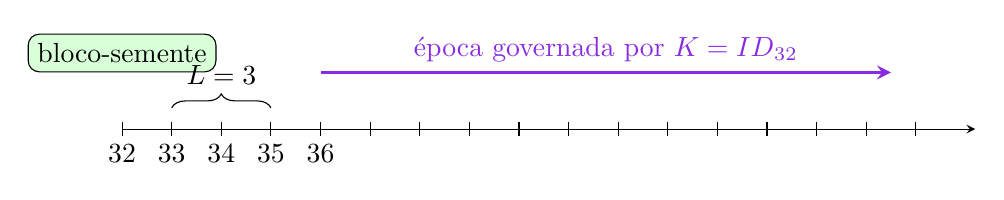
\begin{tikzpicture}[x=.63cm,y=1cm,>=stealth]
 \draw[->] (0,0)--(17.2,0);
 \foreach \x in {0,...,16}{\draw (\x,0.09)--(\x,-.09);}
 \node[below] at (0,-.08) {\(32\)};
 \node[below] at (1,-.08) {\(33\)};
 \node[below] at (2,-.08) {\(34\)};
 \node[below] at (3,-.08) {\(35\)};
 \node[below] at (4,-.08) {\(36\)};
 \node[above,align=center,fill=green!15,draw,rounded corners] at (0,0.72)
   {bloco-semente};
 \draw[decorate,decoration={brace,amplitude=5pt}] (1,.27)--(3,.27)
   node[midway,above=5pt] {\(L=3\)};
 \draw[very thick,BlueViolet,->] (4,.72)--(15.5,.72)
   node[midway,above] {época governada por \(K=\operatorname{ID}_{32}\)};
\end{tikzpicture}
\end{center}

O atraso não torna o bloco-semente impossível de influenciar. Um mineiro pode
tentar reorganizar a cadeia ou reter um bloco, como em qualquer disputa de
prova de trabalho. Torna, porém, dispendioso escolher entre muitas sementes:
quando a chave entra em uso, sessenta e quatro sucessores já investiram
trabalho por cima dela. Abandonar uma semente desfavorável significa abandonar
também essa história.

A mudança a cada 2048 blocos equilibra dois custos. Se \(K\) mudasse a cada
bloco, os mineiros teriam de reconstruir gigabytes de Dataset antes de cada
nova corrida. Se nunca mudasse, uma fábrica poderia ser afinada ou até gravada
para uma tabela eterna. Com blocos de dois minutos, uma época dura cerca de
\begin{align*}
 2048\cdot2\text{ minutos}=4096\text{ minutos}
 \approx 2{,}84\text{ dias}.
\end{align*}
É tempo bastante para amortizar a preparação e curto bastante para que a
memória continue sendo um objecto da cadeia, não mobília de fábrica.


\section{Duas memórias entram numa hospedaria}
\label{sec:randomx-two-memories}

Entram a Cache e o Dataset numa hospedaria. A primeira traz 256 MiB e pede um
quarto; o segundo traz perto de 2080 MiB, exige a cave, a despensa e uma ala do
edifício. O estalajadeiro pergunta qual deles faz o trabalho. «Ambos», responde
a Cache, «mas ele chegou mais cedo.»

A anedota contém a construção inteira. A chave \(K\) alimenta Argon2d, uma
função deliberadamente intensiva em memória \cite{argon2-paper}. Nesta
instanciação, Argon2d preenche 262144 blocos de 1 KiB, numa só pista, e faz
três passagens. O resultado final da fase de preenchimento --- não o resumo
curto normalmente devolvido por uma função de derivação de chave --- é a
Cache:
\begin{align}
 C_K=(C_K[0],C_K[1],\ldots,C_K[m-1]),qquad |C_K|=256\text{ MiB}.
 \label{eq:randomx-cache}
\end{align}

Da Cache nasce o Dataset. Ele contém 34078719 itens de 64 bytes, pouco menos
de 2080 MiB. Cada item pode ser calculado separadamente. Se \(i\) for o seu
índice, escrevemos de forma abstracta
\begin{align}
 D_K[i]=\Phi_K(i,C_K),
 \label{eq:randomx-dataset-item}
\end{align}
onde \(\Phi_K\) faz oito acessos dependentes dos valores anteriores à Cache e,
entre acessos, aplica oito funções de mistura geradas a partir de \(K\). A
especificação chama a essa mistura \emph{SuperscalarHash}. Não é uma nona
função hash criptográfica posta ali por cerimónia: é uma carga longa de
aritmética inteira, sobretudo multiplicações de 64 bits, escolhida para ocupar
as unidades de execução de um processador.

O índice \(i\) entra no estado inicial de forma injectiva dentro do domínio do
Dataset. Depois, cada ronda pode ser vista como
\begin{align*}
 X_0&=\operatorname{enc}(i),\\
 X_{j+1}&=\operatorname{Super}_j(X_j\mathbin{\mathsf{xor}}C_K[a_j]),
       &&j=0,\ldots,7,\\
 D_K[i]&=X_8,
\end{align*}
em que \(a_j\) deriva do próprio estado. Esta notação omite constantes,
ordem de palavras e pormenores de serialização; conserva o facto essencial:
pedir um item obriga a seguir uma cadeia de oito leituras imprevisíveis e oito
misturas dependentes.

Como os itens são independentes entre si, os mineiros podem construir o
Dataset em paralelo quando começa uma época. Como todos derivam de \(K\), não
é preciso publicá-lo nem confiar em quem o preparou. E como \(K\) muda, o
Dataset é uma propriedade que se dissolve periodicamente --- uma forma de
posse privada que nem o mais zeloso cartório conseguiria conservar.


\section{Guardar agora ou calcular depois}
\label{sec:randomx-fast-light}

Há duas maneiras de responder quando a máquina virtual pede \(D_K[i]\):
\begin{description}
 \item[modo completo:] calcular previamente todos os itens e ler o item pedido
 do Dataset em memória;
 \item[modo leve:] guardar apenas \(C_K\) e calcular \(D_K[i]\) nesse momento
 por meio de \(\Phi_K(i,C_K)\).
\end{description}

\begin{center}
\begin{tikzpicture}[>=stealth,node distance=.65cm and 1cm,
  every node/.style={font=\small},
  box/.style={draw,rounded corners,align=center,minimum height=.8cm,
    text width=2.4cm}]
 \node[box,fill=green!12] (cache) {Cache \(C_K\)\\256 MiB};
 \node[box,fill=blue!10,right=2.2cm of cache,yshift=.85cm] (full)
   {Dataset guardado\\\(D_K[i]\) já existe};
 \node[box,fill=yellow!16,right=2.2cm of cache,yshift=-.85cm] (light)
   {cálculo no momento\\\(\Phi_K(i,C_K)\)};
 \node[box,right=2.1cm of full,yshift=-.85cm] (same)
   {o mesmo item\\de 64 bytes};
 \draw[->,thick] (cache)--node[above,sloped]{preparar} (full);
 \draw[->,thick] (cache)--node[below,sloped]{reconstituir} (light);
 \draw[->,thick] (full)--(same);
 \draw[->,thick] (light)--(same);
\end{tikzpicture}
\end{center}

Os modos não são duas provas de trabalho. São duas avaliações da mesma
função. Se a Cache, a chave e o índice forem iguais, a equação
\eqref{eq:randomx-dataset-item} determina os mesmos 64 bytes. Um nó leve pode
portanto verificar um bloco minerado em modo completo; o bloco não anuncia
qual modo foi usado, tal como uma soma não anuncia se foi feita de cabeça ou
num papel.

O modo completo é apropriado à repetição. Paga uma vez a construção do
Dataset e troca cada pedido futuro por uma leitura de DRAM. O modo leve poupa
cerca de oito vezes a memória, mas em cada pedido repete as oito misturas e os
oito acessos à Cache. Uma tentativa executa 16384 voltas da máquina virtual e
faz uma leitura de Dataset por volta. Reconstituir cada item torna a mineração
leve demasiado lenta; para um verificador ocasional, continua a ser uma saída
praticável.

Esta assimetria é subtil. A prova de trabalho clássica é assimétrica entre
\emph{procurar} e \emph{verificar}: o mineiro tenta muitos nonces, o
verificador avalia um. Dentro de uma única avaliação RandomX existe outra
escolha entre memória e tempo. O modo leve é mais lento do que uma avaliação
com Dataset, mas verifica ainda uma vez; o mineiro teria de pagar essa lentidão
milhares de vezes por segundo.


\section{Memória difícil não significa memória abundante}
\label{sec:randomx-memory-hardness}

Exigir dois gigabytes sem mais cuidado não basta. Um adversário pode comprimir
a tabela, guardar apenas uma parte ou construir memória especial junto dos
circuitos de cálculo. Uma função é chamada intensiva em memória quando reduzir
a memória obriga a pagar um aumento desproporcionado de tempo ou trabalho.

Para comparar dispositivos, o desenho de RandomX usa a intuição do produto
área--tempo
\begin{align}
 AT=A\cdot T,
 \label{eq:randomx-area-time}
\end{align}
onde \(A\) aproxima a área de circuito necessária e \(T\) o tempo por
resultado. Um dispositivo que usa metade da memória mas demora dez vezes mais
tem, antes de outros custos, cerca de cinco vezes o produto \(AT\). A medida
não é uma lei física completa: energia, largura de banda, processo de fabrico,
empacotamento e preço de mercado também importam. É uma maneira de impedir que
«menos memória» seja confundido automaticamente com «mais eficiente».

A razão nominal entre os modos foi escolhida em torno de oito:
\begin{align*}
 8\cdot256\text{ MiB}=2048\text{ MiB}.
\end{align*}
O Dataset acrescenta perto de 32 MiB porque o modo leve precisa também da área
e energia das unidades que calculam SuperscalarHash. Assim se chega aos cerca
de 2080 MiB. Os valores foram afinados por medições e modelos de hardware, não
deduzidos de um axioma criptográfico \cite{randomx-design-v1}.

Argon2d protege a própria Cache contra reduções mais agressivas. As referências
de desenho estimam que, com três passagens, reduzir a memória de Argon2d para
metade aumenta por um factor de 3423 o trabalho do melhor compromisso analisado
\cite{memory-hard-tradeoffs,randomx-design-v1}. Esse número pertence a um
modelo de ataque, não é uma garantia de que toda a invenção futura pagará
exactamente 3423. A conclusão robusta é mais sóbria: não há uma interpolação
barata entre guardar a Cache inteira e fingir que ela nunca existiu.

Há, por fim, duas latências diferentes. O Dataset vive em DRAM e custa uma
viagem relativamente longa mas energeticamente natural para um processador.
A Cache pode caber em memória muito mais próxima num ASIC. SuperscalarHash
serve para estragar essa festa: a viagem poupada é substituída por longas
cadeias de dependências e muitas multiplicações. O modo leve não recebe de
presente a vantagem de ter posto 256 MiB dentro do chip.

RandomX não impede que alguém gaste mais capital para construir memória
melhor. Faz com que o custo seja internalizado no dispositivo que procura a
vantagem. É uma defesa muito própria de uma rede sem porteiro: não pergunta
quem fabricou a máquina; altera os preços relativos que ela enfrenta.


\section{A máquina virtual sem linhas de programa}
\label{sec:randomx-vm}

Uma máquina virtual é um acordo sobre uma máquina imaginária. Não interessa
se o nó real tem arquitectura x86, ARM ou RISC-V; interessa que todos concordem
no estado inicial e na transformação causada por cada instrução imaginária.
Um participante pode interpretar as instruções uma a uma ou traduzi-las para
instruções nativas antes de executar. Se a tradução for correcta, o estado
final é o mesmo.

Podemos condensar o estado relevante de RandomX numa tupla
\begin{align}
 \mathcal S=
 (\mathbf r,\mathbf f,\mathbf e,\mathbf a,
  M_1,M_2,M_3,m_a,m_x,\rho),
 \label{eq:randomx-vm-state}
\end{align}
onde:
\begin{itemize}
 \item \(\mathbf r=(r_0,\ldots,r_7)\) contém oito palavras inteiras de 64
 bits;
 \item \(\mathbf f\) e \(\mathbf e\) são dois grupos de quatro registos de
 vírgula flutuante, usados respectivamente por operações aditivas e
 multiplicativas;
 \item \(\mathbf a\) contém quatro valores de vírgula flutuante fixos para o
 programa;
 \item \(M_1\subset M_2\subset M_3\) são três vistas do mesmo Scratchpad;
 \item \(m_a,m_x\) ajudam a escolher os próximos endereços no Dataset; e
 \item \(\rho\) é o modo de arredondamento corrente.
\end{itemize}

Cada membro de \(\mathbf f,\mathbf e,\mathbf a\) contém duas faixas
\emph{binary64}; as operações de vírgula flutuante actuam portanto sobre pares
de números em 128 bits.

Os registos juntos ocupam 256 bytes. O Scratchpad ocupa 2 MiB e funciona como
mesa de trabalho de leitura e escrita. O Dataset é uma biblioteca exterior de
leitura: enorme, comum às tentativas da época e consultada uma vez por volta.

Um programa \(P\) contém 256 instruções e uma configuração. Executar uma
volta é aplicar uma função de transição
\begin{align*}
 \mathcal S_{t+1}=P(\mathcal S_t,D_K),
\end{align*}
e cada programa repete-a 2048 vezes:
\begin{align}
 \mathcal S_{2048}=P^{2048}(\mathcal S_0,D_K).
 \label{eq:randomx-program-iterations}
\end{align}
O expoente aqui significa composição repetida, não elevar bytes a uma
potência. Durante cada volta, endereços derivados do estado seleccionam o que
ler e escrever; por isso, não se pode em geral saltar directamente para
\(\mathcal S_{2048}\).

\subsection{Uma língua em que todo o ruído é uma frase}

Cada instrução ocupa oito bytes. A codificação foi disposta de modo que
\emph{qualquer} palavra de oito bytes seja uma instrução válida e qualquer
sequência dessas palavras seja um programa válido. Não há parêntesis por
fechar, nomes por declarar ou gramática que obrigue a rejeitar bytes até sair
um texto aceitável. Basta produzir bytes pseudo-aleatórios e interpretá-los.

Isto não quer dizer que os programas sejam arbitrários no sentido de poderem
apagar o disco ou telefonar ao vizinho. A linguagem só alcança o estado
\eqref{eq:randomx-vm-state}; não dispõe do sistema operativo. «Todo o ruído é
uma frase» significa apenas que todos os 64 bits de uma palavra recebem uma
interpretação válida dentro dessa cerca.

Os oito bytes escolhem uma operação, registos de origem e destino,
modificadores e uma constante. Há 256 valores possíveis para a parte que
escolhe a operação, distribuídos por 29 espécies de instruções. Dar vários
valores à mesma espécie fixa a sua frequência sem construir uma tabela de
probabilidades separada. Se 16 dos 256 valores representassem uma operação,
por exemplo, ela apareceria em média uma vez por cada 16 instruções.

Não precisamos dos nomes das 29 espécies. Precisamos do que fazem ao custo de
uma máquina:

\begin{center}
\begin{tabular}{>{\raggedright\arraybackslash}p{2.3cm}
                >{\raggedright\arraybackslash}p{4.3cm}
                >{\raggedright\arraybackslash}p{5.5cm}}
\textbf{família}&\textbf{transformações}&\textbf{recurso que põe a trabalhar}\\
\hline
inteira&somas, diferenças, produtos, rotações e XOR&unidades aritméticas,
dependências e cálculo de endereços\\
vírgula flutuante&soma, diferença, produto, divisão e raiz quadrada&unidade de
vírgula flutuante e arredondamento IEEE 754\\
memória&leituras e escritas dependentes do estado&caches, largura de banda e
latência\\
controlo&saltos condicionais raros&execução especulativa e custo de previsões
falhadas\\
\end{tabular}
\end{center}

O repertório é suficientemente próximo das operações nativas para que a
tradução seja rápida, mas suficientemente largo para que um circuito selectivo
não possa ficar apenas com multiplicadores ou apenas com somadores. A
especificação não pretende escrever bons programas. Pretende escrever
programas que sejam maus de uma maneira variada e perfeitamente repetível.


\section{A casa de três andares}
\label{sec:randomx-scratchpad}

O Scratchpad de 2 MiB é uma só sequência de bytes, vista através de três
janelas aninhadas:
\begin{align*}
 |M_1|&=16\text{ KiB},\\
 |M_2|&=256\text{ KiB},\\
 |M_3|&=2\text{ MiB}.
\end{align*}

\begin{center}
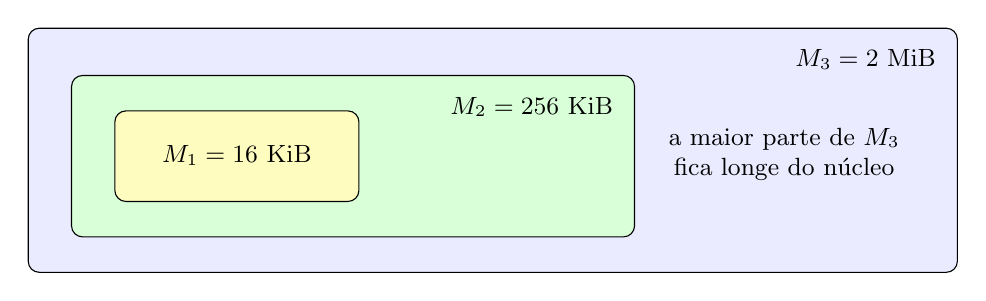
\begin{tikzpicture}[font=\small]
 \draw[fill=blue!8,rounded corners] (0,0) rectangle (11.8,3.1);
 \node[anchor=north east] at (11.65,2.95) {\(M_3=2\) MiB};
 \draw[fill=green!15,rounded corners] (.55,.45) rectangle (7.7,2.5);
 \node[anchor=north east] at (7.55,2.35) {\(M_2=256\) KiB};
 \draw[fill=yellow!25,rounded corners] (1.1,.9) rectangle (4.2,2.05);
 \node at (2.65,1.48) {\(M_1=16\) KiB};
 \node[align=center] at (9.6,1.5) {a maior parte de \(M_3\)\\fica longe do núcleo};
\end{tikzpicture}
\end{center}

Os nomes sugerem as caches físicas L1, L2 e L3 de um processador, mas não
prometem uma correspondência perfeita. A maior parte das instruções de memória
visita as duas janelas pequenas; as leituras dirigidas a \(M_1\) e \(M_2\)
aparecem numa razão de aproximadamente \(3:1\), acompanhando a razão inversa
das latências típicas. Há também dois acessos aleatórios à janela grande por
volta, e certas leituras repetidas de endereço fixo acabam naturalmente
promovidas pela cache física.

No fim de cada volta, o estado de registos é misturado com dois blocos de 64
bytes do Scratchpad e regressa às mesmas zonas. Além disso, instruções de
armazenamento escrevem palavras de oito bytes. A uma volta média correspondem,
segundo a análise de desenho, 504 bytes lidos e 256 escritos, contando acessos
explícitos, movimentos de estado e a linha de Dataset
\cite{randomx-design-v1}.

Como há \(8\cdot2048=16384\) voltas numa tentativa, isto dá aproximadamente
\begin{align*}
 16384\cdot504&=8257536\text{ bytes}=7{,}875\text{ MiB lidos},\\
 16384\cdot256&=4194304\text{ bytes}=4\text{ MiB escritos}.
\end{align*}
Dentro das leituras há precisamente 16384 itens de Dataset de 64 bytes, isto
é, 1 MiB de dados pedidos à memória exterior. O volume não parece enorme; o
custo vem de os endereços serem dependentes do estado e de cada pedido trazer
uma linha curta depois de uma latência longa.

Um varredor sequencial pode mover muitos gigabytes por segundo porque sabe já
qual porta abrir a seguir. RandomX faz perguntas de 64 bytes cujo endereço
nasce da resposta anterior. A largura de banda continua a importar, mas a
latência e o número de bancos de memória tornam-se limites de paralelismo.


\section{O paralelismo que não se vê na página}
\label{sec:randomx-ilp}

Considere-se uma sequência abstracta de quatro operações:
\begin{align*}
 u&=a+b,& v&=c\cdot d,& w&=u\mathbin{\mathsf{xor}}e,& z&=v+w.
\end{align*}
As duas primeiras não dependem uma da outra e podem avançar ao mesmo tempo.
A terceira espera por \(u\); a quarta espera por \(v\) e \(w\). Um processador
\emph{superscalar} possui várias unidades capazes de executar operações no
mesmo ciclo. Um processador \emph{fora de ordem} não fica cerimoniosamente
parado diante de \(w\): adianta qualquer trabalho cujos operandos estejam
prontos.

RandomX gera instruções com dependências e independências misturadas. O
processador corrente investiu enorme área em descobrir estas últimas,
renomear registos e manter muitas operações em voo. Um circuito simples que
execute pela ordem escrita desperdiça essa estrutura. Um ASIC sofisticado
pode reproduzi-la, mas paga pela sofisticação que pretendia evitar.

Os saltos condicionais acrescentam outro embaraço. Cada salto depende de um
valor obtido em execução e tem probabilidade aproximada de \(1/256\) de ser
tomado. Prever «não salta» é quase sempre correcto; quando falha, o trabalho
especulativo é abandonado. As regras de destino impedem ciclos infinitos: o
registo que controla o salto não é alterado no trecho para onde ele volta, de
modo que o mesmo salto não pode continuar a inventar eternidade. Nesta
construção, um salto condicional pode voltar para trás no máximo duas vezes
seguidas.

Uma simulação simplificada publicada com o desenho mediu o programa de 256
instruções em dez processadores imaginários. O modelo mais simples, com uma
unidade aritmética, uma unidade de memória, ordem fixa e sem especulação,
precisou em média de 293 ciclos. Um modelo com quatro unidades aritméticas,
duas de memória, execução fora de ordem e especulação precisou de 64
\cite{randomx-design-v1}. Os números não prevêem um processador comercial;
mostram que os programas recompensam justamente os mecanismos caros que já
existem nos processadores gerais.

Há aqui uma inversão curiosa. Uma função hash fixa costuma ser desenhada para
ter uma estrutura limpa, fácil de analisar e de implementar em paralelo.
RandomX usa primitivas criptográficas limpas nas fronteiras, mas põe no centro
uma pequena desordem administrativa. O caos não é um defeito do programa; é o
produto vendido ao hardware especializado.


\section{Oito programas entram num bar}
\label{sec:randomx-eight-programs}

O empregado olha para os oito programas e pergunta quem paga. O primeiro
aponta para o segundo, o segundo para o terceiro, e assim por diante. O oitavo
aponta para o hash final. Ninguém pode sair discretamente deixando apenas os
programas caros à mesa, porque cada um traz no bolso a semente do seguinte.

Esta corrente resolve o \emph{problema do programa fácil}. O tempo \(T\) de um
programa aleatório não é constante. Programas com mais dependências, divisões
ou acessos infelizes podem demorar mais; as medições de RandomX mostram uma
distribuição próxima de log-normal, com uma cauda de programas lentos. Se cada
programa produzisse sozinho um hash, um mineiro poderia examiná-lo rapidamente
e executar apenas os que favorecessem a sua máquina.

Há duas formas de selecção:
\begin{enumerate}
 \item rejeitar programas previstos como lentos, mesmo numa CPU completa;
 \item construir hardware que execute muito depressa uma fracção da linguagem
 e rejeite tudo o que exige as unidades omitidas.
\end{enumerate}

RandomX encadeia \(N=8\) programas. O primeiro deriva do bloco candidato. O
estado resultante é condensado numa semente de 512 bits que gera o segundo; e
assim sucessivamente:
\begin{align}
 H\longrightarrow P_0\longrightarrow S_1\longrightarrow P_1
 \longrightarrow\cdots\longrightarrow S_7\longrightarrow P_7
 \longrightarrow h_{\rm PoW}.
 \label{eq:randomx-program-chain}
\end{align}
Antes de executar \(P_j\), o mineiro não conhece o estado que gerará
\(P_{j+1}\). Pode abandonar a corrente quando vê um sucessor indesejável, mas
nesse caso perde todos os programas já executados.

\subsection{O preço de ser esquisito}

Suponhamos que uma máquina aceita apenas uma fracção \(Q\) dos programas e
detecta gratuitamente os restantes. Para terminar uma corrente de \(N\)
programas, precisa de obter \(N\) aceitáveis consecutivos. O número médio de
programas efectivamente executados por resultado é
\begin{align}
 E_N(Q)
 &=\frac{1-Q^N}{(1-Q)Q^{N-1}}
  =1+\frac1Q+\frac1{Q^2}+\cdots+\frac1{Q^{N-1}}.
 \label{eq:randomx-filter-cost}
\end{align}
Quando \(Q\to1\), o limite é \(N\), como deve ser para uma máquina que aceita
tudo. Para \(Q=3/4\), obtemos:

\begin{center}
\begin{tabular}{c|c|c}
\(N\)&programas médios por resultado \(E_N(3/4)\)&custo honesto \(N\)\\
\hline
1&1{,}0&1\\
2&2{,}3&2\\
4&6{,}5&4\\
8&27{,}0&8\\
\end{tabular}
\end{center}

Imagine agora que, nos programas aceites, o dispositivo é 50\% mais rápido
do que uma CPU. A sua velocidade relativa, ignorando todos os outros custos,
é
\begin{align*}
 \frac{1{,}5N}{E_N(Q)}.
\end{align*}
Com um só programa e \(Q=3/4\), conserva a vantagem de \(1{,}5\). Com oito,
fica em cerca de
\begin{align*}
 \frac{12}{27}\approx0{,}44.
\end{align*}
O dispositivo brilhante para três quartos da linguagem torna-se menos de
metade tão rápido por resultado. A corrente não torna impossível rejeitar;
torna cara a selectividade.

\subsection{Somar também domestica a cauda}

Se os tempos \(T_1,\ldots,T_N\) fossem independentes, com média \(\mu\) e
variância \(\sigma^2\), o tempo total teria
\begin{align*}
 \operatorname E\!\left[\sum_{j=1}^NT_j\right]&=N\mu,\\
 \operatorname{Var}\!\left(\sum_{j=1}^NT_j\right)&=N\sigma^2.
\end{align*}
O desvio relativo, ou coeficiente de variação, cairia como
\begin{align}
 \frac{\sqrt N\sigma}{N\mu}
 =\frac{1}{\sqrt N}\frac{\sigma}{\mu}.
 \label{eq:randomx-chain-variance}
\end{align}
Os programas reais ligam-se pelas sementes e não são uma experiência ideal de
manual, mas a conta explica a intuição: somar oito durações torna a tentativa
inteira mais regular do que apostar numa duração isolada. Fica menos cauda
onde um seleccionador possa esconder vantagem.


\section{O contabilista de vírgula flutuante}
\label{sec:randomx-floating-point}

Uma regra de consenso deve dar o mesmo resultado em máquinas diferentes. A
vírgula flutuante tem má reputação nesse assunto, não inteiramente imerecida:
compiladores podem trocar a ordem das operações, guardar precisão adicional,
contrair duas operações numa só ou tratar valores excepcionais de maneira
diversa. RandomX usa-a precisamente porque uma unidade de vírgula flutuante é
cara de reproduzir, mas cerca-a com regras destinadas a conservar o consenso.

Um número normal de dupla precisão IEEE 754 tem um bit de sinal \(s\), onze
bits de expoente e 52 bits de fracção. O seu valor é
\begin{align}
 (-1)^s\left(1+\frac{m}{2^{52}}\right)2^{e-1023},
 \label{eq:randomx-binary64}
\end{align}
para os expoentes normais. A recta real é muito mais densa do que o conjunto
destes números. Depois de uma operação, o resultado exacto tem em geral de ser
arredondado para um vizinho representável.

RandomX usa soma, diferença, produto, divisão e raiz quadrada: operações para
as quais o padrão exige arredondamento correcto. Se \(\circ\) representar uma
delas e \(\rho\) o modo de arredondamento, a máquina calcula
\begin{align*}
 x\mathbin{\circ_\rho}y
 =\operatorname{round}_\rho(x\circ y).
\end{align*}
Os quatro modos aparecem nos programas:
\begin{center}
\begin{tabular}{c|l}
\(\rho\)&destino do arredondamento\\
\hline
0&valor representável mais próximo, com desempate para o par\\
1&em direcção a \(-\infty\)\\
2&em direcção a \(+\infty\)\\
3&em direcção a zero\\
\end{tabular}
\end{center}

Não basta ordenar «use IEEE 754». É preciso afastar zonas onde plataformas e
ambientes de execução historicamente discordam. Os operandos introduzidos nas
operações do grupo multiplicativo são forçados a ser positivos e a ter
expoentes entre \(-255\) e \(0\); assim se evitam raízes de números negativos,
divisão por zero e resultados sem número. Valores subnormais são evitados. O
infinito pode surgir, mas surge como uma representação definida e é depois
misturado pelos seus bits.

Os quatro registos aditivos \(\mathbf f\) ficam num domínio em que somar um
operando de módulo maior do que 1 ainda altera bits significativos. Caso
contrário, uma máquina especializada poderia substituir grande parte da
vírgula flutuante por aritmética fixa mais estreita: adicionar uma migalha a
um número gigantesco seria sempre uma operação nula. Outra transformação muda
bits do expoente para tornar essa representação simplificada menos atraente.

Um compilador que resolva associar
\begin{align*}
 (x+y)+z\quad\text{como}\quad x+(y+z)
\end{align*}
pode obter outro resultado, pois cada parêntesis contém um arredondamento. Por
isso a tradução para código nativo não tem liberdade algébrica de compilador
optimista; deve preservar a ordem e o modo prescritos. O intérprete e o
tradutor são dois criados encarregados da mesma contabilidade. Podem andar a
velocidades distintas, mas não lhes é permitido acertar a coluna por intuição.

Esta parte de RandomX é matematicamente relevante justamente porque não há uma
prova abstracta sobre reais. Há uma função finita sobre padrões de 64 bits,
com arredondamento como parte da função. O consenso não pergunta pelo número
ideal \(x\circ y\); pergunta pelos bits de
\(\operatorname{round}_\rho(x\circ y)\).


\section{Da primeira semente ao último bit}
\label{sec:randomx-full-hash}

Podemos agora descrever uma tentativa completa sem uma única linha de
programa. Chamemos \(\mathcal B_{512}\) e \(\mathcal B_{256}\) às versões de
BLAKE2b com saídas de 512 e 256 bits \cite{blake2-paper}. Dado o objecto de
hash \(H\), começa-se por
\begin{align}
 S_0=\mathcal B_{512}(H).
 \label{eq:randomx-initial-seed}
\end{align}

Um gerador rápido baseado em rondas de AES expande \(S_0\) para encher os 2 MiB
do Scratchpad. O seu estado final inicializa outro gerador, com mais rondas por
bloco, que produz a configuração e as 256 instruções do primeiro programa.
As rondas de AES aqui são blocos de construção acelerados por processadores;
não estão a cifrar uma mensagem secreta.

Se \(\operatorname{RF}(\mathcal S_j)\) for o ficheiro de registos de 256 bytes
depois de executar o programa \(P_j\), os sete elos intermédios satisfazem
\begin{align}
 S_{j+1}=\mathcal B_{512}
   \bigl(\operatorname{RF}(\mathcal S_j)\bigr),
 \qquad j=0,\ldots,6.
 \label{eq:randomx-next-program-seed}
\end{align}
Cada \(S_{j+1}\) gera a configuração e o programa seguintes. O Scratchpad não
é reiniciado entre programas; traz consigo as marcas acumuladas da tentativa.

Depois de \(P_7\), uma função baseada em rondas de AES percorre o Scratchpad
inteiro e produz uma impressão de 64 bytes \(A\). Essa impressão substitui o
último quarto do ficheiro de registos antes da condensação final:
\begin{align}
 h_{\rm PoW}=\mathcal B_{256}
 \bigl(\mathbf r\,\|\,\mathbf f\,\|\,\mathbf e\,\|\,A\bigr).
 \label{eq:randomx-final-hash}
\end{align}
O símbolo \(\|\) indica concatenação nas representações fixadas pela
especificação.

\begin{center}
\begin{tikzpicture}[>=stealth,node distance=.5cm and .55cm,
  every node/.style={font=\scriptsize},
  box/.style={draw,rounded corners,align=center,minimum height=.7cm,
    text width=1.75cm,fill=blue!8}]
 \node[box] (H) {\(H\)};
 \node[box,right=of H] (S0) {\(\mathcal B_{512}\)\\\(S_0\)};
 \node[box,right=of S0] (sp) {encher\\Scratchpad};
 \node[box,right=of sp] (p0) {\(P_0^{2048}\)};
 \node[box,right=of p0] (dots) {\(P_1,\ldots,P_6\)};
 \node[box,right=of dots] (p7) {\(P_7^{2048}\)};
 \node[box,below=1cm of p7,xshift=-1.15cm] (rf) {registos\\finais};
 \node[box,text width=1.9cm,below=1cm of p7,xshift=1.15cm] (fp)
   {\(A\): impressão\\\mbox{do Scratchpad}};
 \node[box,below=2.05cm of p7] (out) {\(\mathcal B_{256}\)\\\(h_{\rm PoW}\)};
 \draw[->,thick] (H)--(S0);
 \draw[->,thick] (S0)--(sp);
 \draw[->,thick] (sp)--(p0);
 \draw[->,thick] (p0)--(dots);
 \draw[->,thick] (dots)--(p7);
 \draw[->,thick] (p7)--(rf);
 \draw[->,thick] (p7)--(fp);
 \draw[->,thick] (rf)--(out);
 \draw[->,thick] (fp)--(out);
\end{tikzpicture}
\end{center}

As funções rápidas de uma ou quatro rondas de AES não são usadas como se
fossem, isoladamente, oráculos criptográficos ideais. A primeira recebe uma
semente produzida por BLAKE2b; a impressão do Scratchpad não recebe entrada
livremente escolhida e entra por fim em BLAKE2b. A fronteira criptográfica
forte continua a ser a função hash; as rondas de AES servem para mover e
misturar muitos bytes depressa em hardware comum.

Esta composição também explica por que não se pode calcular apenas os
registos e esquecer a memória. O hash final inclui \(A\), que depende do
Scratchpad inteiro, e os registos dependem de leituras do Dataset e do
Scratchpad ao longo de 16384 voltas. Qualquer atalho deve reproduzir não uma
saída isolada, mas a rede de dependências que a alimentou.


\section{A lotaria depois da máquina}
\label{sec:randomx-lottery}

RandomX termina onde começou o capítulo: num inteiro de 256 bits. Se tratarmos
\(h_{\rm PoW}\) como aproximadamente uniforme em
\(\{0,1,\ldots,2^{256}-1\}\), a condição
\eqref{eq:randomx-difficulty-check} equivale a
\begin{align*}
 h_{\rm PoW}\leq
 \left\lfloor\frac{2^{256}-1}{d}\right\rfloor.
\end{align*}
Logo, a probabilidade de uma tentativa passar é
\begin{align}
 p_d=
 \frac{\left\lfloor(2^{256}-1)/d\right\rfloor+1}{2^{256}}
 \approx\frac1d.
 \label{eq:randomx-success-probability}
\end{align}

Se \(N\) for o número de tentativas até ao primeiro êxito, então, no modelo de
tentativas independentes,
\begin{align*}
 \Pr[N=k]&=(1-p_d)^{k-1}p_d,\\
 \operatorname E[N]&=\frac1{p_d}\approx d,\\
 \operatorname{Var}(N)&=\frac{1-p_d}{p_d^2}.
\end{align*}
O mineiro não prova que executou exactamente \(d\) hashes. Pode acertar à
primeira ou falhar muito depois da média. Prova apenas que apresentou um
bilhete cuja raridade esperada corresponde à dificuldade.

Esta lotaria é cega à marca do processador. Se o mineiro \(i\) produz \(r_i\)
tentativas por segundo e a rede produz
\begin{align*}
 R=\sum_i r_i,
\end{align*}
a probabilidade aproximada de ele encontrar o próximo bloco é \(r_i/R\).
RandomX não altera essa proporcionalidade; tenta alterar quanto custa comprar
cada unidade de \(r_i\) fora de um processador acessível.

O trabalho esperado por bloco continua a ser determinado por \(d\), enquanto
a rede ajusta \(d\) para conservar o intervalo de dois minutos. Uma melhoria
de hardware não faz sair blocos permanentemente mais depressa: aumenta
transitoriamente \(R\), e a dificuldade acompanha-a. A vantagem duradoura do
mineiro é económica, uma fracção maior das recompensas por unidade de custo.


\section{Mercado de hashes, sem ministério dos processadores}
\label{sec:randomx-economics}

Se um bloco paga recompensa base \(B\) e taxas \(F\), o rendimento bruto
esperado do mineiro \(i\) por bloco é aproximadamente
\begin{align}
 \frac{r_i}{R}(B+F).
 \label{eq:randomx-expected-revenue}
\end{align}
Do outro lado estão electricidade, capital, memória, refrigeração, risco e o
uso alternativo da máquina. A concorrência tende a acrescentar potência
enquanto o rendimento marginal esperado justificar o custo marginal. Não há
garantia de equilíbrio instantâneo, nem de que todos paguem a mesma
electricidade; há um incentivo persistente para procurar eficiência.

Um algoritmo que favoreça fortemente um dispositivo escasso pode concentrar
essa procura em fabricantes e operadores com acesso privilegiado. Um algoritmo
favorável a CPUs não distribui magicamente a mineração por uma pessoa e um
portátil. Explorações profissionais continuam a beneficiar de escala,
electricidade barata, memória bem configurada e refrigeração. A afirmação mais
estreita é que o principal bem de capital também tem mercados amplos e usos
alternativos.

Isto muda o custo de entrada e o custo de saída. Um ASIC para uma função
particular pode tornar-se sucata se a moeda mudar de algoritmo; uma CPU pode
ser revendida ou aplicada a outra tarefa. Chamemos \(P\) ao preço de compra,
\(V\) ao valor alternativo depois da mineração e \(L=P-V\) ao capital
efectivamente preso. Para equipamento reaproveitável, \(V\) tende a ser maior
e \(L\) menor. A decisão de entrar exige menos fé numa licença informal
concedida pelo protocolo ao fabricante.

Há também um lado menos romântico. CPUs disseminadas podem ser abusadas por
\emph{malware} ou redes de máquinas comprometidas. RandomX exige memória
substancial para mineração eficiente e deixa actividade pesada mais visível,
mas não converte computadores alheios em propriedade sem dono. Acessibilidade
honesta e acesso criminoso são coisas diferentes; o algoritmo só consegue
moldar custos técnicos, não redigir títulos de propriedade.

Por isso «mais igualitário» deve ser lido como objectivo relativo de desenho,
não como distribuição prometida. O protocolo abre a praça; não reparte as
bancas. Se muitos preferirem delegar a mineração em \emph{pools}, se a energia
for concentrada ou se aparecer hardware superior, a potência pode concentrar-se
mesmo com RandomX.


\section{O que a resistência a ASIC quer dizer}
\label{sec:randomx-asic-resistance}

Há três afirmações de força crescente que não devemos confundir:
\begin{enumerate}
 \item RandomX \textbf{funciona bem em CPUs}: isto pode ser medido;
 \item RandomX \textbf{usa recursos caros de omitir}: isto pode ser modelado,
 comparado e atacado;
 \item RandomX \textbf{impede para sempre qualquer ASIC vantajoso}: isto não
 foi demonstrado e seria uma promessa imprudente.
\end{enumerate}

O termo mais exacto usado no desenho é \emph{vinculação ao dispositivo}. A
função escolhe como referência a classe de processadores gerais existente e
tenta ocupar uma secção transversal da sua arquitectura. Um ASIC pode retirar
funções administrativas, interfaces, compatibilidade e margens que RandomX
não usa. Pode especializar a circulação de dados, escolher tecnologia de
memória diferente e explorar regularidades ainda desconhecidas. Há portanto
espaço para alguma vantagem.

O obstáculo é que a vantagem não deve vir de substituir uma longa função fixa
por uma passadeira de circuito. O dispositivo precisa de:
\begin{itemize}
 \item executar todas as famílias de instruções, sob pena do custo de filtragem
 da equação \eqref{eq:randomx-filter-cost};
 \item manter muitos registos e explorar instruções independentes;
 \item respeitar vírgula flutuante e quatro arredondamentos;
 \item suportar saltos e estados de memória dependentes;
 \item fornecer cerca de dois gigabytes de Dataset por grupo de trabalho
 eficiente, ou pagar a reconstituição leve;
 \item acompanhar uma chave de Dataset que muda com a cadeia.
\end{itemize}

Uma FPGA enfrenta dificuldade semelhante. Reconfigurar fisicamente o circuito
para cada programa demoraria incomparavelmente mais do que a tentativa; manter
um processador virtual dentro da FPGA aproxima-a justamente da máquina geral
que pretendia superar. O espaço de programas deriva de sementes de 512 bits,
portanto contém até \(2^{512}\) possibilidades: não há armazém onde se
preparem antecipadamente circuitos para todas.

Nem todos estes argumentos têm o mesmo estatuto. A igualdade dos modos leve e
completo e a transição da máquina virtual pertencem à especificação. A
uniformidade do resultado depende das propriedades criptográficas das funções
e dos testes. A vantagem futura de hardware depende de tecnologia e economia.
Uma boa exposição deve dizer onde acaba a função e começa a previsão.


\section{Auditorias, versão e fronteira de consenso}
\label{sec:randomx-status}

RandomX foi submetido em 2019 a quatro auditorias independentes, por Trail of
Bits, X41 D-Sec, Kudelski Security e QuarksLab. Os relatórios não registaram
vulnerabilidades críticas; encontraram questões e recomendações que levaram a
alterações no algoritmo e na implementação \cite{randomx-audits}. Isto é
evidência valiosa, não uma canonização. As auditorias têm revisões, plataformas
e âmbitos; não testam todo o silício futuro.

Também há duas espécies de actualização. Uma implementação pode corrigir a
tradução para uma arquitectura sem mudar a função abstracta: os hashes
correctos permanecem os mesmos. Uma versão \emph{algorítmica} muda a função e
portanto exige coordenação de consenso. Se dois nós calcularem funções
RandomX diferentes para o mesmo \((K,H)\), podem discordar sobre
\eqref{eq:randomx-difficulty-check}.

Na fotografia desta edição, o código principal de Monero fixa o compromisso
RandomX 1.2.3, da linha algorítmica 1 \cite{randomx-spec-v1,monero-source-v16}.
O projecto RandomX publicou entretanto a versão algorítmica 2
\cite{randomx-v2-release}. Ela acrescenta trabalho na mistura dos registos de
vírgula flutuante, entre outras alterações, mas não é por isso uma regra activa
de Monero. Substituir a biblioteca por iniciativa individual não seria uma
optimização: seria calcular outra prova de trabalho.

Esta distinção protege o leitor de um hábito perigoso. «Mais recente» é um bom
critério para corrigir uma gralha e um péssimo critério para adivinhar
consenso. A regra activa é a versão que todos os nós devem aplicar àquela
altura. Uma proposta posterior pode merecer estudo sem ser contrabandeada para
o passado.


\section{Uma tentativa, de novo, sem a maquinaria}
\label{sec:randomx-summary}

Reunamos a viagem. Para minerar um bloco à altura \(h\):
\begin{enumerate}
 \item calcula-se \(s(h)\) pela equação \eqref{eq:randomx-seed-height} e toma-se
 como chave \(K\) o ID desse bloco-semente;
 \item de \(K\), Argon2d produz a Cache; dela pode materializar-se o Dataset,
 ou cada item pode ser reconstituído quando pedido;
 \item o objecto de hash do bloco candidato, incluindo o nonce, fornece \(H\)
 e a semente inicial \(S_0=\mathcal B_{512}(H)\);
 \item \(S_0\) enche o Scratchpad e gera o primeiro programa;
 \item oito programas de 256 instruções fazem 2048 voltas cada, lendo o
 Dataset e transformando registos e Scratchpad;
 \item o estado de cada um gera o programa seguinte; depois do oitavo, a
 impressão do Scratchpad e os registos entram em BLAKE2b-256;
 \item o inteiro \(h_{\rm PoW}\) é aceite exactamente quando
 \(h_{\rm PoW}d\leq2^{256}-1\).
\end{enumerate}

O verificador refaz estes passos uma vez. O mineiro volta ao nonce e refaz a
tentativa até a lotaria o favorecer. A dificuldade mede a raridade do bilhete;
RandomX procura determinar que espécie de oficina é mais barata para o
imprimir.

Matematicamente, não encontrámos aqui uma nova hipótese de logaritmo discreto
nem uma prova de conhecimento zero. Encontrámos uma função determinística
composta, uma variável geométrica, cadeias aleatórias, produtos área--tempo,
estados finitos, arredondamentos e modelos de custo. É menos geometria de
curvas e mais aritmética da escassez. Continua a ser matemática, apenas com o
silício sentado à mesa.

\begin{quote}
A Cache lembra a época. O Dataset paga a memória. O Scratchpad lembra a
tentativa. Os oito programas impedem escolher só os dias fáceis. BLAKE2b fecha
a conta; a dificuldade decide se o recibo compra um bloco.
\end{quote}

\label{page:randomx-end}
